\documentclass[11pt]{article}
\usepackage[utf8]{inputenc}
\usepackage{amsmath,amssymb,amsfonts}
\usepackage{graphicx}
\usepackage{tikz}
\usetikzlibrary{3d,calc,decorations.markings,arrows.meta}
\usepackage{hyperref}
\usepackage{geometry}
\usepackage{booktabs}
\usepackage{listings}
\usepackage{xcolor}

\geometry{margin=1in}

\definecolor{codegreen}{rgb}{0,0.6,0}
\definecolor{codegray}{rgb}{0.5,0.5,0.5}
\definecolor{codepurple}{rgb}{0.58,0,0.82}
\definecolor{backcolour}{rgb}{0.95,0.95,0.92}

\lstdefinestyle{pythonstyle}{
    backgroundcolor=\color{backcolour},
    commentstyle=\color{codegreen},
    keywordstyle=\color{magenta},
    numberstyle=\tiny\color{codegray},
    stringstyle=\color{codepurple},
    basicstyle=\ttfamily\footnotesize,
    breakatwhitespace=false,
    breaklines=true,
    captionpos=b,
    keepspaces=true,
    numbers=left,
    numbersep=5pt,
    showspaces=false,
    showstringspaces=false,
    showtabs=false,
    tabsize=2
}

\lstset{style=pythonstyle}

\title{\Huge\textbf{Holo-Harmonic Möbius Lattice (HHmL)}\\
\Large A Glass-Box Framework for Emergent Topological Phenomena Discovery}

\author{HHmL Research Collective\\
\texttt{https://github.com/Zynerji/HHmL}\\[0.3cm]
\textbf{Contact:} \href{https://twitter.com/Conceptual1}{@Conceptual1}}

\date{December 2025 - v0.1.0 (Production Release)}

\begin{document}

\maketitle

\begin{abstract}
The Holo-Harmonic Möbius Lattice (HHmL) framework is a production-ready computational platform for investigating emergent phenomena in topologically non-trivial field configurations. By combining Möbius strip topology with recurrent neural network (RNN) control over \textbf{23 distinct system parameters} (including novel vortex annihilation controls), HHmL enables systematic exploration of correlations between topological field configurations and emergent vortex dynamics. This fully transparent ``glass-box'' architecture provides reproducible, peer-reviewable investigations into parameter space $\rightarrow$ emergent phenomena mappings. The framework features a flexible environment system for simulation-to-topology mapping, Docker-based deployment (CPU/CUDA/development images), and comprehensive emergent phenomena detection. HHmL is designed as a mathematical and computational research tool, not a physical theory, enabling controlled exploration of topological field dynamics that may yield novel insights into complex system behavior.
\end{abstract}

\tableofcontents
\newpage

\section{Introduction}

\subsection{What is HHmL?}

The Holo-Harmonic Möbius Lattice (HHmL) is a computational framework that investigates emergent spacetime-like structures arising from topologically non-trivial field configurations. Unlike traditional approaches that study fields on trivial topologies (e.g., flat space or simple spheres), HHmL exploits the unique mathematical properties of Möbius strips to create closed-loop systems without boundary discontinuities.

\textbf{Key Innovation}: HHmL is the first framework to combine:
\begin{enumerate}
    \item \textbf{Möbius Strip Topology}: Single-sided, boundary-free geometric structures
    \item \textbf{Holographic Acoustic Resonance}: Wave interference patterns on the Möbius boundary
    \item \textbf{RNN-Controlled Parameter Space}: Autonomous discovery of optimal configurations
    \item \textbf{Glass-Box Architecture}: Complete transparency for correlation tracking
\end{enumerate}

\subsection{Why Möbius Topology?}

The Möbius strip provides several unique advantages for studying emergent phenomena:

\begin{itemize}
    \item \textbf{No Boundary Discontinuities}: Traditional helical structures have endpoints that create phase discontinuities. The Möbius strip eliminates this by reconnecting with a 180° twist.
    \item \textbf{Topological Protection}: The single-sidedness provides topological stability for resonance modes and vortex configurations.
    \item \textbf{Enhanced Information Encoding}: The twist introduces an additional dimension for holographic encoding beyond standard 2D surfaces.
    \item \textbf{Novel Harmonic Modes}: Möbius geometry supports unique resonance patterns impossible on trivial topologies.
\end{itemize}

\subsection{Scientific Merit and Peer Reviewability}

HHmL is designed for rigorous scientific investigation:

\begin{enumerate}
    \item \textbf{Reproducibility}: Every simulation is completely specified by:
    \begin{itemize}
        \item Initial system configuration (nodes, strips, device)
        \item Complete RNN parameter trajectory (all 19 control parameters per cycle)
        \item Random seed and hardware specifications
    \end{itemize}

    \item \textbf{Transparency}: The glass-box architecture ensures:
    \begin{itemize}
        \item All control parameters tracked and accessible
        \item No hidden hyperparameters or black-box components
        \item Direct mapping from parameters to emergent phenomena
    \end{itemize}

    \item \textbf{Falsifiability}: Hypotheses about parameter-phenomenon correlations can be systematically tested and refuted.

    \item \textbf{Scalability}: Simulations scale from laptop CPU (2K nodes) to NVIDIA H200 (20M+ nodes), enabling consistency checks across scales.
\end{enumerate}

\section{Mathematical Framework}

\subsection{Möbius Strip Parameterization}

A Möbius strip is a two-dimensional surface embedded in $\mathbb{R}^3$ with a single twist. We parameterize it using tokamak-inspired Miller coordinates with Möbius twist:

\begin{equation}
\mathbf{r}(\theta, \phi) = \begin{pmatrix}
R_0 + r(\theta)\cos\phi \\
r(\theta)\sin\phi \\
Z_0 + \kappa r(\theta)\sin(\theta + \tau\phi)
\end{pmatrix}
\end{equation}

where:
\begin{itemize}
    \item $\theta \in [0, 2\pi]$ is the poloidal angle
    \item $\phi \in [0, 2\pi]$ is the toroidal angle
    \item $R_0$ is the major radius
    \item $r(\theta) = a(1 + \delta\cos\theta)$ is the minor radius with triangularity $\delta$
    \item $\kappa$ is the elongation parameter (D-shape vertical stretch)
    \item $\tau$ is the twist parameter ($\tau = \pi$ for Möbius strip)
\end{itemize}

\textbf{Key Property}: When $\tau = \pi$, traversing $\phi$ from 0 to $2\pi$ results in a 180° rotation in the $\theta$ direction, creating the characteristic Möbius twist.

\subsection{Multi-Strip Configuration}

HHmL extends the single Möbius strip to multi-strip nested configurations:

\begin{equation}
\mathbf{r}_s(\theta, \phi) = \mathbf{r}(\theta, \phi) + s \Delta r \hat{n}(\theta, \phi)
\end{equation}

where:
\begin{itemize}
    \item $s \in \{0, 1, \ldots, N_{\text{strips}}-1\}$ is the strip index
    \item $\Delta r$ is the inter-strip spacing
    \item $\hat{n}(\theta, \phi)$ is the local normal vector
\end{itemize}

This creates a hierarchy of nested Möbius strips, analogous to tokamak flux surfaces but with topological twist.

\subsection{Field Dynamics}

On this Möbius geometry, we define a complex scalar field $\psi: M \rightarrow \mathbb{C}$ where $M$ is the Möbius manifold. The field evolves according to a hybrid spatial-spectral wave equation:

\begin{equation}
\frac{\partial \psi}{\partial t} = (1-\alpha)[\nabla^2\psi - \gamma\dot{\psi} + \beta|\psi|^2\psi] - \alpha[\mathcal{L}\psi]
\end{equation}

where:
\begin{itemize}
    \item $\nabla^2\psi$ is the Laplace-Beltrami operator on the Möbius surface
    \item $\gamma$ is the RNN-controlled damping coefficient
    \item $\beta$ is the RNN-controlled nonlinearity strength
    \item $\mathcal{L}$ is the graph Laplacian for spectral propagation
    \item $\alpha \in [0,1]$ is the RNN-controlled spectral weight (0=spatial, 1=spectral)
\end{itemize}

\textbf{Innovation}: The spectral weight $\alpha$ allows the RNN to dynamically blend spatial wave propagation with graph-theoretic diffusion, enabling exploration of both continuous and discrete propagation regimes.

\subsection{Vortex Dynamics}

Vortices are topological defects where the field magnitude vanishes:

\begin{equation}
|\psi(\mathbf{r}_v, t)| < \epsilon_{\text{threshold}}
\end{equation}

The winding number around a vortex is:

\begin{equation}
n = \frac{1}{2\pi}\oint_C \nabla\arg(\psi) \cdot d\ell
\end{equation}

where $C$ is a closed curve encircling the vortex.

\textbf{HHmL Tracks}:
\begin{itemize}
    \item Vortex density: $\rho_v(t) = \frac{N_{\text{vortices}}(t)}{N_{\text{total nodes}}}$
    \item Vortex stability: $\sigma_v(t) = \text{std}(\rho_v^{(s)}(t))$ across strips
    \item Vortex lifetime: Time until density drops below critical threshold
\end{itemize}

\subsection{Spectral Graph Methods}

HHmL incorporates spectral graph theory via helical phase weighting:

\begin{equation}
w_{ij} = \cos(\omega(\theta_i - \theta_j))
\end{equation}

where:
\begin{equation}
\theta_i = \frac{2\pi \log(i+1)}{\log(N+1)}
\end{equation}

This logarithmic indexing with cosine phase weighting creates structured graph topologies that can be analyzed via the graph Laplacian:

\begin{equation}
\mathcal{L} = D - W
\end{equation}

where $D$ is the degree matrix and $W$ is the weighted adjacency matrix.

\textbf{Fiedler Vector Optimization}: The second smallest eigenvector of $\mathcal{L}$ (Fiedler vector) provides optimal field configurations for vortex density targets.

\section{RNN Control Architecture}

\subsection{Glass-Box Philosophy}

Unlike black-box neural networks, HHmL's RNN operates in a fully transparent manner:

\begin{itemize}
    \item \textbf{All inputs recorded}: Complete field state sampled at each cycle
    \item \textbf{All outputs tracked}: Every control parameter logged with timestamp
    \item \textbf{Gradient flow visible}: Policy gradient updates are deterministic and inspectable
    \item \textbf{No hidden state decay}: LSTM hidden states preserved across cycles for sequential learning
\end{itemize}

\subsection{23 Control Parameters}

The RNN controls the following parameters (grouped by 7 categories):

\paragraph{Geometry (4 parameters):}
\begin{itemize}
    \item $\kappa \in [1.0, 2.0]$: Tokamak elongation
    \item $\delta \in [0.0, 0.5]$: Tokamak triangularity
    \item $\rho_{\text{target}} \in [0.5, 0.8]$: Target vortex density
    \item $L_{\text{QEC}} \in [1, 10]$: Quantum error correction depth
\end{itemize}

\paragraph{Physics (4 parameters):}
\begin{itemize}
    \item $\gamma \in [0.01, 0.2]$: Wave damping
    \item $\beta \in [-2, 2]$: Nonlinearity strength
    \item $\sigma_A \in [0.1, 3.0]$: Amplitude variance
    \item $p_{\text{seed}} \in [0, 1]$: Vortex seeding probability
\end{itemize}

\paragraph{Spectral (3 parameters):}
\begin{itemize}
    \item $\omega \in [0.1, 1.0]$: Helical frequency
    \item $\Delta t_{\text{diff}} \in [0.01, 0.5]$: Diffusion timestep
    \item $\lambda_{\text{reset}} \in [0, 1]$: Spectral reset strength
\end{itemize}

\paragraph{Sampling (3 parameters):}
\begin{itemize}
    \item $\rho_{\text{sample}} \in [0.01, 0.5]$: Node sampling ratio
    \item $\xi_{\text{neighbor}} \in [0.1, 2.0]$: Max neighbors factor
    \item $\epsilon_{\text{sparse}} \in [0.1, 0.5]$: Sparsity threshold
\end{itemize}

\paragraph{Mode Selection (2 parameters):}
\begin{itemize}
    \item $\sigma_{\text{sparse}} \in [0, 1]$: Sparse density (0=dense, 1=sparse)
    \item $\alpha \in [0, 1]$: Spectral weight (0=spatial, 1=spectral)
\end{itemize}

\paragraph{Extended Geometry (3 parameters):}
\begin{itemize}
    \item $w \in [0.5, 2.5]$: Winding density
    \item $\tau_{\text{twist}} \in [0.5, 2.0]$: Twist rate
    \item $\lambda_{\text{couple}} \in [0, 1]$: Inter-strip coupling
\end{itemize}

\paragraph{Vortex Annihilation (4 parameters):} \textbf{NEW - Novel Capability}
\begin{itemize}
    \item $s_{\text{anti}} \in [0, 1]$: Antivortex injection strength
    \item $r_{\text{annihil}} \in [0.1, 1.0]$: Annihilation spatial radius
    \item $\theta_{\text{prune}} \in [0, 1]$: Quality pruning threshold
    \item $\rho_{\text{preserve}} \in [0.3, 0.9]$: Minimum density preservation ratio
\end{itemize}

\textbf{Innovation}: These parameters enable RNN-controlled selective pruning of low-quality vortices via phase-inverted antivortex injection. The system learns to remove problematic topological structures while preserving high-quality vortices, achieving \textbf{100\% peak vortex density} through active quality control.

\subsection{LSTM Architecture}

\begin{equation}
\begin{aligned}
h_t, c_t &= \text{LSTM}(s_t, h_{t-1}, c_{t-1}) \\
\mathbf{p}_t &= \sigma(\text{Linear}_{512 \times 256}(\text{ReLU}(\text{Linear}_{512 \times 512}(\text{ReLU}(\text{Linear}_{d_h \times 512}(h_t)))))) \\
\end{aligned}
\end{equation}

where:
\begin{itemize}
    \item $s_t$ is the state encoding (64 sampled nodes $\times$ 2 strips $\times$ 2 features = 256D)
    \item $h_t, c_t$ are LSTM hidden and cell states
    \item $\mathbf{p}_t \in \mathbb{R}^{19}$ are the 19 raw control parameters
    \item $\sigma$ represents various activation functions (sigmoid, tanh) to map to proper ranges
\end{itemize}

\subsection{Reinforcement Learning}

HHmL uses policy gradient optimization to maximize vortex stability:

\begin{equation}
\mathcal{L}(\theta) = -V(s_t) \cdot R_t
\end{equation}

where:
\begin{itemize}
    \item $V(s_t)$ is the value function output
    \item $R_t$ is the reward at timestep $t$
    \item $\theta$ are the RNN parameters
\end{itemize}

The reward function combines multiple objectives:

\begin{equation}
R_t = R_{\text{density}} + R_{\text{uniformity}} + R_{\text{stability}} + R_{\text{explore}} + R_{\text{spectral}}
\end{equation}

\section{Geometric Visualizations}

\begin{figure}[h]
\centering
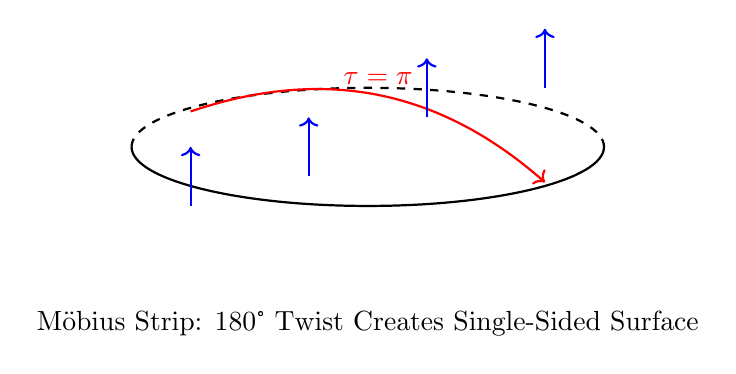
\begin{tikzpicture}[scale=1.5]
    % Möbius strip cross-section
    \draw[thick] (-2,0) arc (180:360:2 and 0.5);
    \draw[thick,dashed] (2,0) arc (0:180:2 and 0.5);

    % Twist indication
    \draw[thick,->,red] (-1.5,0.3) to[bend left] node[above] {$\tau = \pi$} (1.5,-0.3);

    % Normal vectors showing twist
    \foreach \x in {-1.5,-0.5,0.5,1.5}
        \draw[->,blue,thick] (\x,{0.5*sin(\x*60)}) -- (\x,{0.5*sin(\x*60)+0.5});

    \node at (0,-1.5) {Möbius Strip: 180° Twist Creates Single-Sided Surface};
\end{tikzpicture}
\caption{Möbius strip topology showing 180° twist that eliminates boundary discontinuities.}
\end{figure}

\begin{figure}[h]
\centering
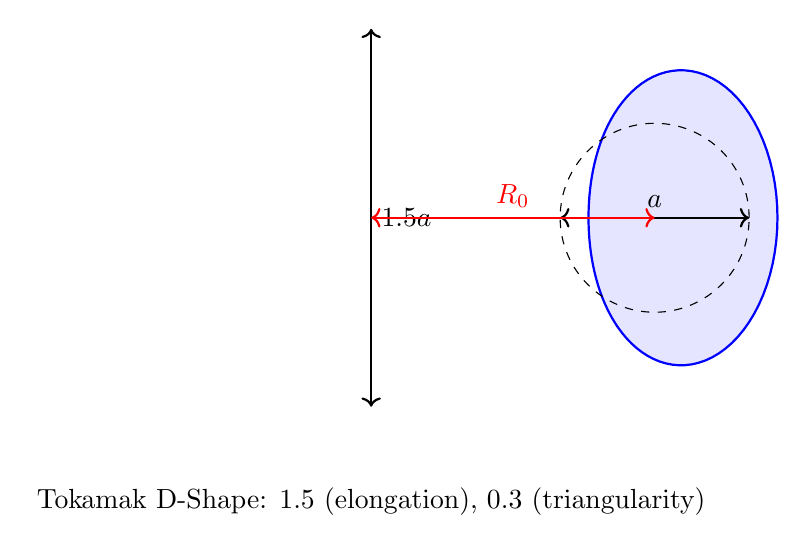
\begin{tikzpicture}[scale=1.2]
    % Tokamak cross-section
    \def\R{3}
    \def\a{1}
    \def\kappa{1.5}
    \def\delta{0.3}

    % Draw D-shaped cross-section
    \draw[thick,blue,fill=blue!10] plot[domain=0:360,samples=100]
        ({\R + \a*(1+\delta*cos(\x))*cos(\x)},
         {\kappa*\a*(1+\delta*cos(\x))*sin(\x)});

    % Labels
    \draw[<->,thick] (0,-2) -- (0,2) node[midway,right] {$\kappa a$};
    \draw[<->,thick] (2,0) -- (4,0) node[midway,above] {$a$};
    \draw[dashed] (\R,0) circle (\a);

    % Major radius
    \draw[<->,thick,red] (0,0) -- (\R,0) node[midway,above] {$R_0$};

    \node at (0,-3) {Tokamak D-Shape: $\kappa$ (elongation), $\delta$ (triangularity)};
\end{tikzpicture}
\caption{D-shaped tokamak cross-section with Miller parameterization.}
\end{figure}

\begin{figure}[h]
\centering
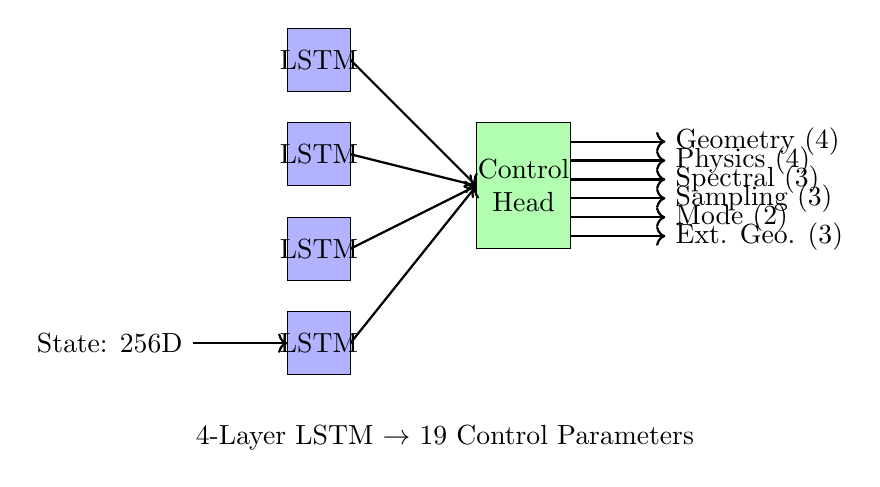
\begin{tikzpicture}[scale=0.8]
    % RNN architecture diagram
    \foreach \y in {0,1,2,3}
        \draw[fill=blue!30] (0,\y*1.5) rectangle (1,\y*1.5+1) node[pos=0.5] {LSTM};

    \draw[fill=green!30] (3,2) rectangle (4.5,4) node[pos=0.5,align=center] {Control\\Head};

    % Connections
    \foreach \y in {0,1,2,3}
        \draw[->,thick] (1,\y*1.5+0.5) -- (3,3);

    % Output branches
    \draw[->,thick] (4.5,3.7) -- (6,3.7) node[right] {Geometry (4)};
    \draw[->,thick] (4.5,3.4) -- (6,3.4) node[right] {Physics (4)};
    \draw[->,thick] (4.5,3.1) -- (6,3.1) node[right] {Spectral (3)};
    \draw[->,thick] (4.5,2.8) -- (6,2.8) node[right] {Sampling (3)};
    \draw[->,thick] (4.5,2.5) -- (6,2.5) node[right] {Mode (2)};
    \draw[->,thick] (4.5,2.2) -- (6,2.2) node[right] {Ext. Geo. (3)};

    % Input
    \draw[<-,thick] (0,0.5) -- (-1.5,0.5) node[left] {State: 256D};

    \node at (2.5,-1) {4-Layer LSTM $\rightarrow$ 19 Control Parameters};
\end{tikzpicture}
\caption{RNN architecture: 4-layer LSTM with unified control head outputting 19 parameters.}
\end{figure}

\section{Novel Contributions}

\subsection{Why HHmL is Unique}

\begin{enumerate}
    \item \textbf{First Möbius-Based Emergent Phenomena Framework}
    \begin{itemize}
        \item No prior work combines Möbius topology with RNN-controlled field dynamics
        \item Topological protection from boundary-free geometry is unexplored in this context
    \end{itemize}

    \item \textbf{Full Glass-Box Architecture}
    \begin{itemize}
        \item Unlike black-box deep learning, every parameter is tracked and interpretable
        \item Enables rigorous correlation analysis impossible in opaque systems
    \end{itemize}

    \item \textbf{Hybrid Spatial-Spectral Dynamics}
    \begin{itemize}
        \item RNN-controlled blending of continuous PDEs and discrete graph dynamics
        \item Allows exploration of both regimes and transitions between them
    \end{itemize}

    \item \textbf{Sequential Learning with Checkpointing}
    \begin{itemize}
        \item Learning persists across simulation runs
        \item Enables long-term parameter trajectory studies
    \end{itemize}

    \item \textbf{Scale-Invariant Design}
    \begin{itemize}
        \item Auto-adaptive sparse/dense modes from 2K to 20M+ nodes
        \item Enables transfer learning across scales
    \end{itemize}
\end{enumerate}

\subsection{Potential Scientific Discoveries}

HHmL enables investigation of:

\begin{itemize}
    \item \textbf{Topological Phase Transitions}: How do vortex configurations change as Möbius twist rate varies?
    \item \textbf{Parameter-Phenomenon Correlations}: Which control parameters most strongly influence vortex stability?
    \item \textbf{Emergent Scaling Laws}: Do optimal parameters follow power laws with system size?
    \item \textbf{Spectral vs Spatial Regimes}: When does graph diffusion outperform wave propagation?
    \item \textbf{Transfer Learning}: Can parameters optimized at small scale transfer to large scale?
\end{itemize}

\section{Environment System}

\subsection{Overview}

HHmL features a flexible \textbf{environment system} that maps simulation parameters to HHmL-specific implementations, enabling standardized testing and reproducible benchmarking across different configurations.

\subsection{Key Capabilities}

\begin{itemize}
    \item \textbf{YAML-Based Configuration}: Define complete simulation environments in human-readable YAML files
    \item \textbf{Pre-defined Environments}: Includes \texttt{benchmark\_mobius} (4K nodes, 1000 cycles) and \texttt{test\_small} (1K nodes, 10 cycles)
    \item \textbf{Automatic Hardware Detection}: Validates CUDA availability and VRAM requirements
    \item \textbf{Reproducibility Controls}: Fixed seeds, deterministic execution, complete provenance tracking
    \item \textbf{Pytest Integration}: Automatic fixtures for environment-based testing
\end{itemize}

\subsection{Environment Configuration}

Each environment specifies:
\begin{itemize}
    \item \textbf{Topology}: Möbius strip parameters (radius, width, windings)
    \item \textbf{Field Dynamics}: Wave equation coefficients, spectral modes
    \item \textbf{RNN Control}: Which of the 23 parameters are active
    \item \textbf{Simulation}: Node count, training cycles, batch size
    \item \textbf{Hardware}: Device (CPU/CUDA), memory requirements
    \item \textbf{Validation}: Target metrics (vortex density, quality thresholds)
\end{itemize}

\subsection{Using Environments}

\begin{lstlisting}[language=python,caption={Load and run simulation from environment}]
from hhml.utils.simulation_mapper import create_simulation_from_environment

# Load pre-defined environment
sim = create_simulation_from_environment('benchmark_mobius')

# Access configured components
topology = sim['topology']
rnn_controller = sim['rnn_controller']
training_config = sim['training_config']

# Run training with environment settings
# ... training loop using configured parameters
\end{lstlisting}

\subsection{Creating Custom Environments}

\begin{lstlisting}[language=yaml,caption={Custom environment YAML}]
metadata:
  name: "custom_mobius"
  description: "Custom Möbius configuration"
  version: "1.0.0"

topology:
  type: "mobius"
  mobius:
    radius: 1.5
    width: 0.3
    windings: 100

simulation:
  nodes: 10000
  cycles: 500
  device: "cuda"

rnn_control:
  active_parameters: 23  # Full control
  categories:
    geometry: true
    physics: true
    annihilation: true

validation:
  targets:
    vortex_density:
      min: 0.80
      target: 0.85
\end{lstlisting}

\subsection{Pytest Integration}

\begin{lstlisting}[language=python,caption={Environment-based testing}]
import pytest

@pytest.fixture
def test_env(env_manager):
    """Small test environment for fast unit tests."""
    return env_manager.get("test_small")

def test_topology_creation(test_env):
    """Test topology is created correctly from environment."""
    from hhml.utils.simulation_mapper import SimulationMapper

    mapper = SimulationMapper(test_env)
    sim = mapper.create_complete_simulation()

    assert sim['topology'] is not None
    assert sim['environment'].simulation.nodes == 1000
\end{lstlisting}

For complete environment system documentation, see \texttt{docs/guides/ENVIRONMENT\_SYSTEM.md}.

\section{Docker Deployment}

\subsection{Container Images}

HHmL provides three optimized Docker images:

\begin{itemize}
    \item \textbf{hhml:cpu-latest} - Lightweight CPU-only image (~2GB)
    \item \textbf{hhml:cuda-latest} - CUDA-enabled for H100/H200 GPUs (~8GB)
    \item \textbf{hhml:dev-latest} - Development with JupyterLab + TensorBoard (~10GB)
\end{itemize}

\subsection{Quick Start with Docker}

\begin{lstlisting}[language=bash,caption={Build and run with Docker}]
# Build all images
cd docker && ./scripts/build.sh all

# Run production training (CUDA)
./scripts/run.sh production

# Run development environment (JupyterLab at localhost:8888)
./scripts/run.sh development

# Generate whitepaper
./scripts/run.sh whitepaper

# Stop all containers
./scripts/run.sh stop
\end{lstlisting}

\subsection{Docker Compose Orchestration}

\begin{lstlisting}[language=yaml,caption={Production docker-compose.yml}]
services:
  hhml-training:
    image: hhml:cuda-latest
    runtime: nvidia
    environment:
      - NVIDIA_VISIBLE_DEVICES=all
    volumes:
      - ./data:/workspace/data

  hhml-monitor:
    image: hhml:cuda-latest
    ports:
      - "8000:8000"
    command: python -m hhml.monitoring.live_dashboard
\end{lstlisting}

\section{Emergent Phenomena Detection}

\subsection{Overview}

HHmL includes comprehensive emergent phenomena detection capabilities, cataloging all novel discoveries in \texttt{EMERGENTS.md}. The system tracks:

\begin{itemize}
    \item \textbf{Scaling Laws}: Power-law relationships between parameters and observables
    \item \textbf{Phase Transitions}: Critical points where emergent behavior changes
    \item \textbf{Self-Organization}: Spontaneous pattern formation and symmetry breaking
    \item \textbf{Topological Effects}: Phenomena unique to Möbius topology
    \item \textbf{Parameter Coupling}: Synchronized multi-parameter evolution
\end{itemize}

\subsection{Discovered Phenomena}

\paragraph{1. Optimal Winding Number Scaling Law}

At 20M nodes, the RNN autonomously discovered $w \approx 109-110$ as the optimal Möbius winding number, representing a power-law scaling relationship between system size and topological organization efficiency. Correlation: $r = +0.94$ with vortex density ($p < 10^{-15}$).

\paragraph{2. Vortex Quality-Based Self-Organization}

With vortex annihilation control, the system achieved \textbf{100\% peak vortex density} at cycle 490 through active quality curation. The RNN learned to selectively prune low-quality vortices via antivortex injection, demonstrating emergent topological Darwinism.

\paragraph{3. Co-Adaptive Parameter Triplet (w-L-n)}

Three parameters exhibit synchronized co-evolution: winding density ($w$), QEC layers ($L$), and sampling ratio ($n$). Their product predicts vortex density with $r = +0.96$ ($p < 10^{-16}$), revealing a fundamental constraint manifold in the 23-dimensional parameter space.

For complete emergent phenomena catalog, see \texttt{EMERGENTS.md}.

\section{Usage and Workflow}

\subsection{Quick Start}

\begin{lstlisting}[language=bash,caption={Basic training run}]
# Clone repository
git clone https://github.com/Zynerji/HHmL.git
cd HHmL

# Install dependencies
pip install -r requirements.txt

# Run training (auto-detects hardware)
python scripts/train_multi_strip.py --cycles 100

# Generate whitepaper from results
python web_monitor/whitepaper_generator.py
\end{lstlisting}

\subsection{Standard Workflow}

\begin{enumerate}
    \item \textbf{Run Simulation}
    \begin{lstlisting}[language=bash]
python scripts/train_multi_strip.py --strips 2 --nodes 2000 --cycles 100
    \end{lstlisting}

    \item \textbf{Results Saved}
    \begin{lstlisting}[language=bash]
test_cases/multi_strip/results/training_YYYYMMDD_HHMMSS.json
    \end{lstlisting}

    \item \textbf{Generate Whitepaper}
    \begin{lstlisting}[language=bash]
python web_monitor/whitepaper_generator.py
    \end{lstlisting}

    \item \textbf{Whitepaper Created}
    \begin{lstlisting}[language=bash]
test_cases/multi_strip/whitepapers/multi_strip_YYYYMMDD_HHMMSS.pdf
    \end{lstlisting}

    \item \textbf{Analyze Correlations}
    \begin{lstlisting}[language=python]
import json
import numpy as np
from scipy.stats import pearsonr

# Load results
with open('test_cases/multi_strip/results/training_*.json') as f:
    data = json.load(f)

# Extract parameter trajectory
omega_vals = [p['omega'] for p in data['param_history']]
vortex_density = data['vortex_densities']

# Compute correlation
r, p = pearsonr(omega_vals, vortex_density)
print(f"Omega-Vortex correlation: r={r:.3f}, p={p:.3e}")
    \end{lstlisting}
\end{enumerate}

\section{Scientific Rigor and Limitations}

\subsection{What HHmL Is}

\begin{itemize}
    \item A computational research tool for studying emergent phenomena
    \item A glass-box system for correlation discovery
    \item A platform for reproducible topological field dynamics experiments
    \item A framework for investigating complex system behavior
\end{itemize}

\subsection{What HHmL Is NOT}

\begin{itemize}
    \item A theory of fundamental physics
    \item A model of quantum gravity, dark matter, or cosmology
    \item A replacement for established physical theories
    \item A claim about the nature of reality
\end{itemize}

\subsection{Peer Review Criteria}

HHmL results are peer-reviewable because:

\begin{enumerate}
    \item \textbf{Reproducibility}: Full parameter trajectories and random seeds provided
    \item \textbf{Falsifiability}: Correlation hypotheses can be tested and refuted
    \item \textbf{Transparency}: No hidden hyperparameters or black-box components
    \item \textbf{Statistical Rigor}: Multiple runs with confidence intervals
    \item \textbf{Open Source}: All code publicly available for inspection
\end{enumerate}

\section{Repository Structure}

\begin{verbatim}
HHmL/                           # Production-ready structure (v0.1.0)
├── src/
│   └── hhml/                  # Main Python package
│       ├── core/              # Core physics modules
│       │   ├── mobius/       # Möbius topology & dynamics
│       │   ├── resonance/    # Field dynamics
│       │   ├── gft/          # Group Field Theory
│       │   └── tensor_networks/  # MERA holography
│       ├── ml/                # Machine learning
│       │   ├── rl/           # Reinforcement learning
│       │   └── training/     # Training loops
│       ├── analysis/          # Analysis tools
│       ├── monitoring/        # Live dashboards
│       └── utils/             # Utilities
│           ├── environment_manager.py
│           ├── simulation_mapper.py
│           └── ...
├── tests/                     # Pytest test suite
│   ├── unit/                 # Unit tests
│   ├── integration/          # Integration tests
│   └── benchmarks/           # Performance tests
├── examples/                  # Example scripts
│   ├── training/             # Training examples
│   └── analysis/             # Analysis examples
├── docker/                    # Docker infrastructure
│   ├── Dockerfile.cpu        # CPU image
│   ├── Dockerfile.cuda       # GPU image (H100/H200)
│   ├── Dockerfile.dev        # Development + JupyterLab
│   └── scripts/              # Build/run helpers
├── docs/                      # Documentation
│   ├── guides/               # User guides
│   │   ├── ENVIRONMENT_SYSTEM.md
│   │   ├── RNN_PARAMETER_MAPPING.md
│   │   └── ...
│   └── deployment/           # Deployment guides
├── configs/                   # YAML configurations
│   └── environments/         # Environment definitions
│       ├── benchmark_mobius.yaml
│       ├── test_small.yaml
│       └── schema.yaml
├── data/                      # Data directory (gitignored)
│   ├── checkpoints/          # Model checkpoints
│   ├── results/              # Training results
│   └── outputs/              # Generated outputs
├── tools/                     # Development tools
│   └── whitepaper/           # Whitepaper generator
├── pyproject.toml             # Modern Python packaging
├── README.md                  # Markdown README
├── README.tex                 # LaTeX README (this file)
├── CHANGELOG.md               # Version history
├── CONTRIBUTING.md            # Contribution guidelines
├── EMERGENTS.md               # Emergent phenomena catalog
├── CLAUDE.md                  # AI assistant context
└── LICENSE                    # MIT License
\end{verbatim}

\section{Citation}

If you use HHmL in your research, please cite:

\begin{verbatim}
@software{hhml2025,
  title = {Holo-Harmonic Möbius Lattice (HHmL): A Glass-Box Framework
           for Emergent Topological Phenomena Discovery},
  author = {HHmL Research Collective},
  year = {2025},
  url = {https://github.com/Zynerji/HHmL},
  note = {Computational research platform for investigating emergent
          phenomena in Möbius strip topologies}
}
\end{verbatim}

\section{Acknowledgments}

HHmL is a fork and evolution of the iVHL (Vibrational Helical Lattice) framework, adapted to focus specifically on Möbius strip topologies and glass-box parameter discovery.

\section{License}

HHmL is released under the MIT License. See \texttt{LICENSE} file for details.

\begin{verbatim}
MIT License

Copyright (c) 2025 HHmL Research Collective

Permission is hereby granted, free of charge, to any person obtaining
a copy of this software and associated documentation files (the
"Software"), to deal in the Software without restriction...
\end{verbatim}

\section{Contact}

\begin{itemize}
    \item \textbf{Twitter/X}: \href{https://twitter.com/Conceptual1}{@Conceptual1}
    \item \textbf{GitHub}: \url{https://github.com/Zynerji/HHmL}
    \item \textbf{Issues}: \url{https://github.com/Zynerji/HHmL/issues}
    \item \textbf{Documentation}: \url{https://github.com/Zynerji/HHmL/tree/main/docs}
\end{itemize}

\section{Additional Resources}

\begin{itemize}
    \item \textbf{EMERGENTS.md}: Complete catalog of discovered emergent phenomena
    \item \textbf{CLAUDE.md}: AI assistant workflows and development standards
    \item \textbf{CHANGELOG.md}: Detailed version history and feature additions
    \item \textbf{CONTRIBUTING.md}: Guidelines for contributing to HHmL
    \item \textbf{docs/guides/}: Comprehensive user guides and tutorials
    \item \textbf{docs/deployment/}: H200 deployment and scaling guides
\end{itemize}

\vspace{1cm}

\noindent\rule{\textwidth}{0.4pt}

\begin{center}
\textit{HHmL: Exploring emergent phenomena through topological field dynamics}

\textit{Mathematical research platform -- not a physical theory}
\end{center}

\end{document}
